\subsection{Simultaneous Localisation and Mapping (SLAM)}
In the SLAM problem, we assume we don't have the knowledge of neither the map $\vec M$, nor the vehicle states $\vec x_1, \dotsc, \vec x_T$. We want to figure out $p(\vec x_t, \vec M \mid \vec z_{1:t}, \vec u_{1:t})$. The graphical model is as follows
\begin{figure}[!htb]
\centering
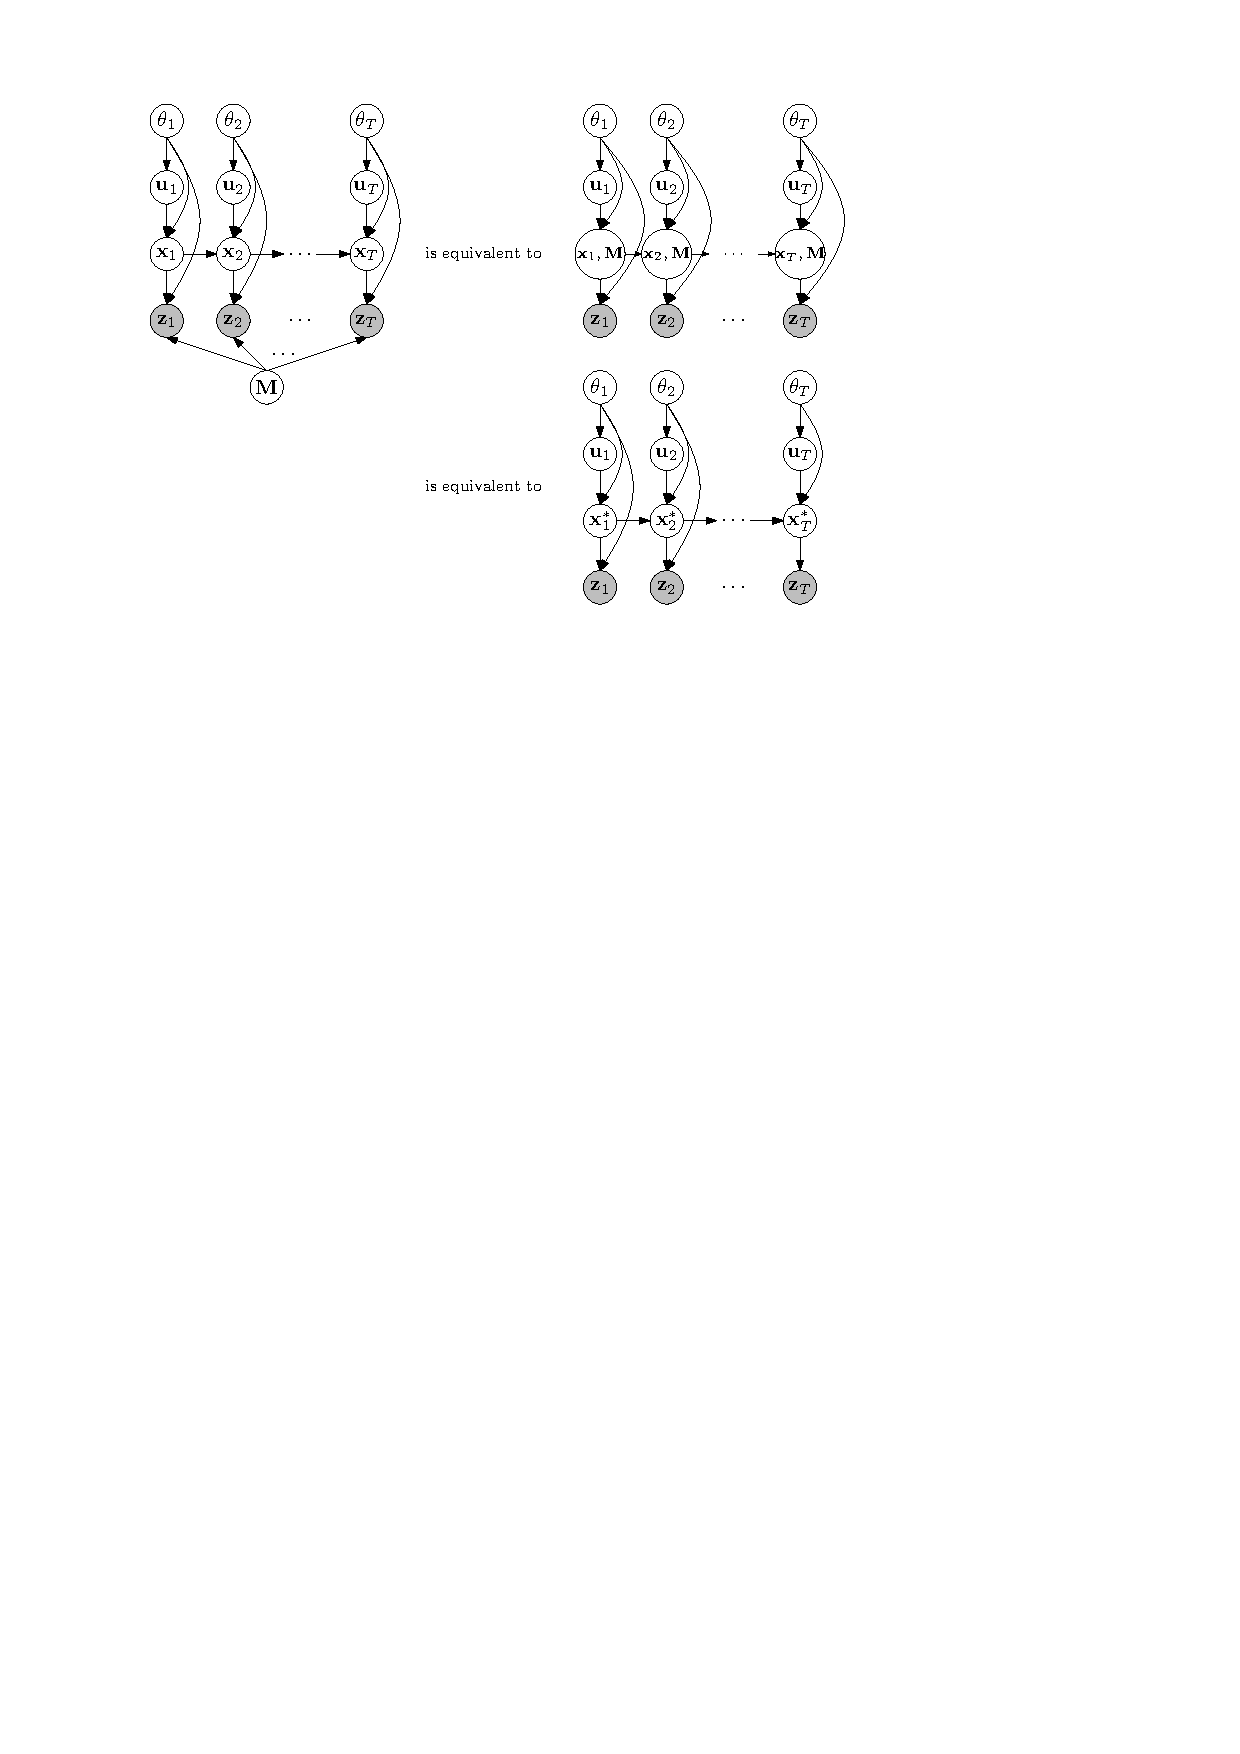
\includegraphics[scale=1]{models/kf/figures/kf-slam}
\caption{Probabilistic Graphical Model for the Kalman Filter for SLAM.}
\label{fig:models/kf/figures/kf-slam}
\end{figure}

The graphical model is almost similar to the one in the case of mapping (Figure~\ref{fig:models/kf/figures/kf-map}), the only difference being that $\vec x_1, \dotsc, \vec x_T$ are unobserved. We also group the $\vec x$'s and $\vec M$ together, for $t = 1, \dotsc, T$:
\begin{equation}
	\vec x_t^\ast =
		\begin{bmatrix}
			\vec x_t \\
			\vec M
		\end{bmatrix}
\end{equation}

Similarly to the mapping case, the model can be described, for $t = 1, \dotsc, T$, by the following equations:
\begin{align}
	\vec x_t^\ast 	&= \vec g^\ast(\vec x_{t - 1}^\ast, \vec u_t) + \vec \epsilon_t^\ast \\
	\vec z_t 		&= \vec h^\ast(\vec x_t^\ast, \vec u_t) + \vec \delta_t^\ast
\end{align}
We need to characterise $\vec g^\ast(\vec x^\ast, \vec u)$, $\vec \epsilon_t^\ast$, $\vec h^\ast(\vec x^\ast, \vec u)$, and $\vec \delta_t^\ast$ to describe the EKF algorithm fully.

\subsubsection{The transition model}
The transition model is defined for (part of) the state
\begin{align}
	\vec x_t = 
		\begin{bmatrix}
			x_t \\
			y_t \\
			\theta_t
		\end{bmatrix}
\end{align}
which contains the position and orientation of the vehicle (note the slightly overloaded notation of $\vec x_t$ and $x_t$). The transition model is then described by
\begin{align}
	\vec g^\ast(\vec x^\ast_{t - 1}, \vec u_t) = \vec x^\ast_{t - 1} + 
		\begin{bmatrix}
			-\frac{v_t}{\omega_t} \sin(\theta_{t - 1}) + \frac{v_t}{\omega_t} \sin(\theta_{t - 1} + \omega_t \Delta t) \\
			\frac{v_t}{\omega_t} \cos(\theta_{t - 1}) - \frac{v_t}{\omega_t} \cos(\theta_{t - 1} + \omega_t \Delta t) \\
			\omega_t \Delta t \\
			0 \\
			\vdots \\
			0
		\end{bmatrix}
\end{align}
where $\vec u_t = (v_t, \omega_t)^T$ contains translational and rotational velocities. The zeros arise because the map doesn't change.

\subsubsection{The observation model}
The observation model is defined for the observation variable is the same as the one in the Localisation case, described in the Subsubsection~\ref{subsubsec:models/kf/localisation/obs}, in Equations~\eqref{eqn:models/kf/localisation/obs} and \eqref{eqn:models/kf/localisation/obs2}. The observation model is then
\begin{align}
	\vec h^\ast(\vec x^\ast_t, \vec u_t) =
									\begin{bmatrix}
										\|\vec m_{c_{t, 1}} - (x_t, y_t)^T\| \\
										\arctan\left((m_{c_{t, 1}, y} - y_t) / (m_{c_{t, 1}, x} - x_t) \right) - \theta_t \\
										\vdots \\
										\|\vec m_{c_{t, \ell}} - (x_t, y_t)^T\| \\
										\arctan\left((m_{c_{t, \ell}, y} - y_t) / (m_{c_{t, \ell}, x} - x_t) \right) - \theta_t \\
										\vdots \\
										\|\vec m_{c_{t, L}} - (x_t, y_t)^T\| \\
										\arctan\left((m_{c_{t, L}, y} - y_t) / (m_{c_{t, L}, x} - x_t) \right) - \theta_t
									\end{bmatrix}
\end{align}
and
\begin{align}
	\vec R_t = \diag(\sigma^2_r, \sigma^2_\phi, \dotsc, \sigma^2_r, \sigma^2_\phi) \in \mathbb R^{2L \times 2L}
\end{align}
Note that the observation model is very similar to the one in the Localisation case, the only differences being grouping of $\vec x, \vec M$ into $\vec x^\ast$.